\chapter{Análisis}

En esta sección se cubren los requisitos funcionales y no funcionales para el desarrollo del proyecto. Se describen los casos de uso y se detallan los escenarios y actores del sistema.

\newpage
 
\section{Requisitos funcionales}

La calidad del software puede medirse en concordancia con los requisitos funcionales y de rendimiento que se establezcan, con las características intrínsecas que se esperan de cualquier software desarrollado de manera profesional. Los requisitos funcionales son aquellos que definen como debe comportarse el sistema, es decir, las funciones específicas que se esperan que cumplan con las necesidades finales del usuario \cite{Veloz_Segura_2022}.\newline

A continuación se describirán los requisitos funcionales, clasificados según su gestión principal, a fin de facilitar la comprensión clara de las funcionalidades que la plataforma debe incluir.

\subsection{Gestión de usuarios}

En este apartado se describen todas las funcionalidades relativas a los usuarios. Nótese que al referirnos al término ``usuario'' nos referimos a cualquier persona que haga uso de la plataforma, ya sea un administrador, un profesor o un alumno.
\newcounter{rfCounter}
\setcounter{rfCounter}{1}

\begin{table}[H]
    \centering
    \begin{tabular}{|p{4cm}|p{7cm}|}
    \hline
    \multicolumn{2}{|c|}{\textbf{RF\therfCounter\ - Registro de Usuario}} \\ \hline
    \textbf{Descripción} & Permite a un nuevo usuario registrarse en el sistema. \\ \hline
    \textbf{Datos de entrada} & Correo institucional. \\ \hline
    \textbf{Datos de salida} & Confirmación de registro. \\ \hline
    \end{tabular}
    \caption{RF\therfCounter\ - Registro de Usuario.}
    \stepcounter{rfCounter}
\end{table}

\begin{table}[H]
    \centering
    \begin{tabular}{|p{4cm}|p{7cm}|}
    \hline
    \multicolumn{2}{|c|}{\textbf{RF\therfCounter\ - Inicio de Sesión}} \\ \hline
    \textbf{Descripción} & Permite a un usuario identificarse y acceder a sus datos. \\ \hline
    \textbf{Datos de entrada} & Credenciales del usuario. \\ \hline
    \textbf{Datos de salida} & Avatar del usuario en la pantalla de inicio y acceso a la opción de consultar sus horarios. \\ \hline
    \end{tabular}
    \caption{RF\therfCounter\ - Inicio de Sesión.}
    \stepcounter{rfCounter}
\end{table}

\begin{table}[H]
    \centering
    \begin{tabular}{|p{4cm}|p{7cm}|}
    \hline
    \multicolumn{2}{|c|}{\textbf{RF\therfCounter\ - Baja de Usuario}} \\ \hline
    \textbf{Descripción} & Permite eliminar a un usuario del sistema y a sus datos asociados. \\ \hline
    \textbf{Datos de entrada} & Credenciales del usuario. \\ \hline
    \textbf{Datos de salida} & Confirmación de baja. \\ \hline
    \end{tabular}
    \caption{RF\therfCounter\ - Baja de Usuario.}
    \stepcounter{rfCounter}
\end{table}

\subsection{Gestión de Calendarios}

En este apartado se describe la gestión de los calendarios semanales creados por el usuario con el fin de organizar su matrícula o su horario de clases. Nótese que al referirnos al término ``combinación'' estamos haciendo referencia a uno de los calendarios semanales generados por el sistema con las asignaturas y grupos seleccionados por el usuario. 

\begin{table}[H]
    \centering
    \begin{tabular}{|p{4cm}|p{7cm}|}
    \hline
    \multicolumn{2}{|c|}{\textbf{RF\therfCounter\ - Seleccionar Grado}} \\ \hline
    \textbf{Descripción} & Permite al usuario seleccionar el grado de la UGR del que querrá organizar sus asignaturas. \\ \hline
    \textbf{Datos de entrada} & Lista de grados de la UGR. \\ \hline
    \textbf{Datos de salida} & Grado seleccionado. \\ \hline
    \end{tabular}
    \caption{RF\therfCounter\ - Seleccionar Grado.}
    \stepcounter{rfCounter}
\end{table}


\begin{table}[H]
    \centering
    \begin{tabular}{|p{4cm}|p{7cm}|}
    \hline
    \multicolumn{2}{|c|}{\textbf{RF\therfCounter\ - Seleccionar Curso}} \\ \hline
    \textbf{Descripción} & Permite al usuario seleccionar un curso académico. \\ \hline
    \textbf{Datos de entrada} & Lista de cursos del grado seleccionado. \\ \hline
    \textbf{Datos de salida} & Curso seleccionado. \\ \hline
    \end{tabular}
    \caption{RF\therfCounter\ - Seleccionar Curso.}
    \stepcounter{rfCounter}
\end{table}

\begin{table}[H]
    \centering
    \begin{tabular}{|p{4cm}|p{7cm}|}
    \hline
    \multicolumn{2}{|c|}{\textbf{RF\therfCounter\ - Seleccionar Cuatrimestre}} \\ \hline
    \textbf{Descripción} & Permite al usuario seleccionar un cuatrimestre del curso académico seleccionado. \\ \hline
    \textbf{Datos de entrada} & Lista de cuatrimestres del curso y grado seleccionado. \\ \hline
    \textbf{Datos de salida} & Cuatrimestre seleccionado. \\ \hline
    \end{tabular}
    \caption{RF\therfCounter\ - Seleccionar Cuatrimestre.}
    \stepcounter{rfCounter}
\end{table}

\begin{table}[H]
    \centering
    \begin{tabular}{|p{4cm}|p{7cm}|}
    \hline
    \multicolumn{2}{|c|}{\textbf{RF\therfCounter\ - Seleccionar Asignatura}} \\ \hline
    \textbf{Descripción} & Permite al usuario seleccionar una asignatura para incluirla en la planificación de su calendario semanal. \\ \hline
    \textbf{Datos de entrada} & Lista de asignaturas del grado seleccionado. \\ \hline
    \textbf{Datos de salida} & Asignatura seleccionada. \\ \hline
    \end{tabular}
    \caption{RF\therfCounter\ - Seleccionar Asignatura.}
    \stepcounter{rfCounter}
\end{table}

\begin{table}[H]
    \centering
    \begin{tabular}{|p{4cm}|p{7cm}|}
    \hline
    \multicolumn{2}{|c|}{\textbf{RF\therfCounter\ - Seleccionar Grupo}} \\ \hline
    \textbf{Descripción} & Permite al usuario seleccionar un grupo de teoría a planificar para la asignatura que ha previamente seleccionado. \\ \hline
    \textbf{Datos de entrada} & Lista de grupos de la asignatura seleccionada. \\ \hline
    \textbf{Datos de salida} & Grupo seleccionado. \\ \hline
    \end{tabular}
    \caption{RF\therfCounter\ - Seleccionar Grupo.}
    \stepcounter{rfCounter}
\end{table}

\begin{table}[H]
    \centering
    \begin{tabular}{|p{4cm}|p{7cm}|}
    \hline
    \multicolumn{2}{|c|}{\textbf{RF\therfCounter\ - Seleccionar Combinación}} \\ \hline
    \textbf{Descripción} & Permite al usuario seleccionar una combinación de las generadas por el sistema con su selección de asignaturas y grupos. \\ \hline
    \textbf{Datos de entrada} & Lista de combinaciones generadas. \\ \hline
    \textbf{Datos de salida} & Combinación seleccionada. \\ \hline
    \end{tabular}
    \caption{RF\therfCounter\ - Seleccionar Calendario.}
    \stepcounter{rfCounter}
\end{table}

\begin{table}[H]
    \centering
    \begin{tabular}{|p{4cm}|p{7cm}|}
    \hline
    \multicolumn{2}{|c|}{\textbf{RF\therfCounter\ - Descargar Combinación}} \\ \hline
    \textbf{Descripción} & Permite al usuario descargar la combinación deseada en formato PDF. \\ \hline
    \textbf{Datos de entrada} & Combinación seleccionada. \\ \hline
    \textbf{Datos de salida} & Calendario de la combinación seleccionada en formato PDF. \\ \hline
    \end{tabular}
    \caption{RF\therfCounter\ - Descargar Combinación.}
    \stepcounter{rfCounter}
\end{table}

\begin{table}[H]
    \centering
    \begin{tabular}{|p{4cm}|p{7cm}|}
    \hline
    \multicolumn{2}{|c|}{\textbf{RF\therfCounter\ - Guardar Calendario}} \\ \hline
    \textbf{Descripción} & Permite al usuario guardar la combinación seleccionada en el sistema para consultarla posteriormente. \\ \hline
    \textbf{Datos de entrada} & Combinación seleccionada. \\ \hline
    \textbf{Datos de salida} & Combinación guardada como calendario. \\ \hline
    \end{tabular}
    \caption{RF\therfCounter\ - Guardar Calendario.}
    \stepcounter{rfCounter}
\end{table}

\begin{table}[H]
    \centering
    \begin{tabular}{|p{4cm}|p{7cm}|}
    \hline
    \multicolumn{2}{|c|}{\textbf{RF\therfCounter\ - Consultar Calendario}} \\ \hline
    \textbf{Descripción} & Permite al usuario consultar sus calendarios finales guardados. \\ \hline
    \textbf{Datos de entrada} & Lista de calendarios guardados. \\ \hline
    \textbf{Datos de salida} & Calendario guardado seleccionado. \\ \hline
    \end{tabular}
    \caption{RF\therfCounter\ - Consultar Calendario.}
    \stepcounter{rfCounter}
\end{table}

\section{Requisitos no funcionales}

Los requisitos no funcionales son aquellos que no se refieren específicamente a la funcionalidad de un sistema. Imponen restricciones sobre el producto que se está desarrollando y el proceso de desarrollo, y especifican restricciones externas que debe cumplir el producto \cite{nonFR}.

\newcounter{nrfCounter}
\setcounter{nrfCounter}{1}

\begin{table}[H]
    \centering
    \begin{tabular}{|p{4cm}|p{7cm}|}
    \hline
    \multicolumn{2}{|c|}{\textbf{RNF\thenrfCounter\ - Usabilidad}} \\ \hline
    \textbf{Descripción} & La plataforma debe ser fácil e intuitiva para los usuarios. \\ \hline
    \textbf{Criterios} & Interfaz de usuario sencilla y autoexplicativa. \\ \hline
    \end{tabular}
    \caption{RNF\thenrfCounter\ - Usabilidad.}
    \stepcounter{nrfCounter}
\end{table}

\begin{table}[H]
    \centering
    \begin{tabular}{|p{4cm}|p{7cm}|}
    \hline
    \multicolumn{2}{|c|}{\textbf{RNF\thenrfCounter\ - Rendimiento}} \\ \hline
    \textbf{Descripción} & La plataforma debe responder con rapidez a las consultas del usuario. \\ \hline
    \textbf{Criterios} & Tiempos de respuesta rápidos para las peticiones. \\ \hline
    \end{tabular}
    \caption{RNF\thenrfCounter\ - Rendimiento.}
    \stepcounter{nrfCounter}
\end{table}

\begin{table}[H]
    \centering
    \begin{tabular}{|p{4cm}|p{7cm}|}
    \hline
    \multicolumn{2}{|c|}{\textbf{RNF\thenrfCounter\ - Eficiencia}} \\ \hline
    \textbf{Descripción} & La plataforma debe reducir el tiempo que el usuario tardaría en hacer su calendario semanal manualmente. \\ \hline
    \textbf{Criterios} & Proceso rápido y automático de generación del calendario. \\ \hline
    \end{tabular}
    \caption{RNF\thenrfCounter\ - Eficiencia.}
    \stepcounter{nrfCounter}
\end{table}

\begin{table}[H]
    \centering
    \begin{tabular}{|p{4cm}|p{7cm}|}
    \hline
    \multicolumn{2}{|c|}{\textbf{RNF\thenrfCounter\ - Compatibilidad}} \\ \hline
    \textbf{Descripción} & La plataforma funcionará correctamente independientemente del navegador o dispositivo usado. \\ \hline
    \textbf{Criterios} & React permite un diseño responsive y React Native permite desplegar archivos APK para Android y archivos para iOS  . \\ \hline
    \end{tabular}
    \caption{RNF\thenrfCounter\ - Compatibilidad.}
    \stepcounter{nrfCounter}
\end{table}

\begin{table}[H]
    \centering
    \begin{tabular}{|p{4cm}|p{7cm}|}
    \hline
    \multicolumn{2}{|c|}{\textbf{RNF\thenrfCounter\ - Mantenibilidad}} \\ \hline
    \textbf{Descripción} & La plataforma facilitará las actualizaciones y el desarrollo de su contenido. \\ \hline
    \textbf{Criterios} & La documentación y el código de la plataforma se desarrollarán de forma clara para facilitar su entendimiento y posterior actualización. \\ \hline
    \end{tabular}
    \caption{RNF\thenrfCounter\ - Mantenibilidad.}
    \stepcounter{nrfCounter}
\end{table}

\section{Modelo de Caso de Uso}

Los casos de uso son una secuencia de eventos que en conjunto, conducen a un sistema haciendo algo útil. Describen las diferentes formas en que los usuarios interaccionan con el mismo y como este les responde. Son una herramienta fundamental para la comprensión de los requisitos funcionales y ayudan a entender las funcionalidades esperadas del sistema y las partes implicadas \cite{bittner2003use}.

\subsection{Actores del Sistema}

La interacción con la plataforma se basa en dos tipos de actores: los usuarios sin registrar y los usuarios registrados. El acceso no está restringido a usuarios registrados, pero estos últimos disponen de funcionalidades adicionales.

\begin{enumerate}
    \item \textbf{Usuario genérico}: Son los usuarios que acceden a la plataforma para generar sus calendarios semanales y es principalmente a quien va dirigida la plataforma. Pueden seleccionar el grado, curso, cuatrimestre, asignaturas y grupos que desean incluir en su calendario semanal. Consultar los calendarios generados, descargarlos en formato PDF y guardarlos en la plataforma para consultarlos posteriormente.
    \item \textbf{Usuario Registrado}: Son los usuarios que han completado el proceso de registro en la plataforma. Tienen acceso a las mismas funcionalidades que los usuarios genéricos, pero además pueden guardar sus calendarios semanales en la plataforma para consultarlos posteriormente.
\end{enumerate}

\subsection{Escenarios de Casos de Uso}

\newcounter{ccCounter}
\setcounter{ccCounter}{1}
% Ajustar el espacio entre elementos flotantes
\setlength{\textfloatsep}{5pt plus 1.0pt minus 2.0pt} % Espacio entre el texto y los elementos flotantes
\setlength{\floatsep}{5pt plus 1.0pt minus 2.0pt} % Espacio entre dos elementos flotantes
\setlength{\intextsep}{5pt plus 1.0pt minus 2.0pt} % Espacio entre el texto y los elementos flotantes insertados en el texto


\begin{table}[H]
    \centering
    \begin{tabular}{|p{4cm}|p{7cm}|}
    \hline
    \multicolumn{2}{|c|}{\textbf{CU\theccCounter\ - Registrar Usuario}} \\ \hline
    \textbf{Actores} & Usuario Genérico. \\ \hline
    \textbf{Precondiciones} & El actor no está registrado en el sistema. \\ \hline
    \textbf{Postcondiciones} & El actor está registrado en el sistema. \\ \hline
    \textbf{Flujo principal} & \begin{minipage}[t]{\linewidth}
        \vspace{1pt}
        \begin{enumerate}
            \setlength{\itemsep}{0pt}
            \setlength{\parskip}{0pt}
            \setlength{\parsep}{0pt}
            \item El actor accede a la plataforma.
            \item El actor ingresa su correo institucional.
            \item El sistema envía un correo de confirmación al correo institucional del actor.
            \item El actor confirma su registro en la plataforma.
            \item El sistema registra al actor en la plataforma.
        \end{enumerate}
        \vspace{1pt}
    \end{minipage} \\ \hline  
    \end{tabular}
    \caption{CU\theccCounter\ - Registrar Usuario.}
    \stepcounter{ccCounter}
\end{table}

\begin{table}[H]
    \centering
    \begin{tabular}{|p{4cm}|p{7cm}|}
    \hline
    \multicolumn{2}{|c|}{\textbf{CU\theccCounter\ - Autenticar Usuario}} \\ \hline
    \textbf{Actores} & Usuario Registrado. \\ \hline
    \textbf{Precondiciones} & El actor está registrado en el sistema. \\ \hline
    \textbf{Postcondiciones} & El actor está autenticado en el sistema. \\ \hline
    \textbf{Flujo principal} & \begin{minipage}[t]{\linewidth}
        \vspace{1pt}
        \begin{enumerate}
            \setlength{\itemsep}{0pt}
            \setlength{\parskip}{0pt}
            \setlength{\parsep}{0pt}
            \item El actor accede a la plataforma.
            \item El actor ingresa sus credenciales.
            \item El sistema valida sus credenciales.
            \item El sistema muestra el avatar del actor en la pantalla de inicio y le da acceso a la opción de consultar sus horarios.
        \end{enumerate}
        \vspace{1pt}
    \end{minipage} \\ \hline  
    \end{tabular}
    \caption{CU\theccCounter\ - Autenticar Usuario.}
    \stepcounter{ccCounter}
\end{table}

\begin{table}[H]
    \centering
    \begin{tabular}{|p{4cm}|p{7cm}|}
    \hline
    \multicolumn{2}{|c|}{\textbf{CU\theccCounter\ - Eliminar Usuario}} \\ \hline
    \textbf{Actores} & Usuario Registrado. \\ \hline
    \textbf{Precondiciones} & El actor está registrado en el sistema. \\ \hline
    \textbf{Postcondiciones} & El actor no está registrado en el sistema. \\ \hline
    \textbf{Flujo principal} & \begin{minipage}[t]{\linewidth}
        \vspace{1pt}
        \begin{enumerate}
            \setlength{\itemsep}{0pt}
            \setlength{\parskip}{0pt}
            \setlength{\parsep}{0pt}
            \item El actor accede a la plataforma.
            \item El actor selecciona la opción de eliminar su cuenta.
            \item El sistema solicita confirmación al actor.
            \item El actor confirma la eliminación de su cuenta.
            \item El sistema elimina al actor de la plataforma y sus datos asociados.
        \end{enumerate}
        \vspace{1pt}
    \end{minipage} \\ \hline  
    \end{tabular}
    \caption{CU\theccCounter\ - Eliminar Usuario.}
    \stepcounter{ccCounter}
\end{table}

\begin{table}[H]
    \centering
    \begin{tabular}{|p{4cm}|p{7cm}|}
    \hline
    \multicolumn{2}{|c|}{\textbf{CU\theccCounter\ - Seleccionar Grado}} \\ \hline
    \textbf{Actores} & Usuario Genérico y Usuario Registrado. \\ \hline
    \textbf{Precondiciones} & El actor accede a la plataforma. \\ \hline
    \textbf{Postcondiciones} & Se muestran los datos del grado seleccionado. \\ \hline
    \textbf{Flujo principal} & \begin{minipage}[t]{\linewidth}
        \vspace{1pt}
        \begin{enumerate}
            \setlength{\itemsep}{0pt}
            \setlength{\parskip}{0pt}
            \setlength{\parsep}{0pt}
            \item El actor accede a la plataforma.
            \item El sistema muestra la lista de grados disponibles.
            \item El actor selecciona el grado de interés.
            \item El sistema muestra los datos del grado seleccionado.
        \end{enumerate}
        \vspace{1pt}
    \end{minipage} \\ \hline  
    \end{tabular}
    \caption{CU\theccCounter\ - Seleccionar Grado.}
    \stepcounter{ccCounter}
\end{table}

\begin{table}[H]
    \centering
    \begin{tabular}{|p{4cm}|p{7cm}|}
    \hline
    \multicolumn{2}{|c|}{\textbf{CU\theccCounter\ - Seleccionar Curso}} \\ \hline
    \textbf{Actores} & Usuario Genérico y Usuario Registrado. \\ \hline
    \textbf{Precondiciones} & El actor accede a la plataforma. \\ \hline
    \textbf{Postcondiciones} & Se muestran los datos del curso seleccionado. \\ \hline
    \textbf{Flujo principal} & \begin{minipage}[t]{\linewidth}
        \vspace{1pt}
        \begin{enumerate}
            \setlength{\itemsep}{0pt}
            \setlength{\parskip}{0pt}
            \setlength{\parsep}{0pt}
            \item El actor accede a la plataforma.
            \item El sistema muestra la lista de grados disponibles.
            \item El actor selecciona el grado de interés.
            \item El sistema muestra la lista de cursos disponibles.
            \item El actor selecciona el curso de interés.
            \item El sistema muestra los datos del curso seleccionado.
        \end{enumerate}
        \vspace{1pt}
    \end{minipage} \\ \hline  
    \end{tabular}
    \caption{CU\theccCounter\ - Seleccionar Curso.}
    \stepcounter{ccCounter}
\end{table}

\begin{table}[H]
    \centering
    \begin{tabular}{|p{4cm}|p{7cm}|}
    \hline
    \multicolumn{2}{|c|}{\textbf{CU\theccCounter\ - Seleccionar Cuatrimestre}} \\ \hline
    \textbf{Actores} & Usuario Genérico y Usuario Registrado. \\ \hline
    \textbf{Precondiciones} & El actor accede a la plataforma. \\ \hline
    \textbf{Postcondiciones} & Se muestran los datos del cuatrimestre seleccionado. \\ \hline
    \textbf{Flujo principal} & \begin{minipage}[t]{\linewidth}
        \vspace{1pt}
        \begin{enumerate}
            \setlength{\itemsep}{0pt}
            \setlength{\parskip}{0pt}
            \setlength{\parsep}{0pt}
            \item El actor accede a la plataforma.
            \item El sistema muestra la lista de grados disponibles.
            \item El actor selecciona el grado de interés.
            \item El sistema muestra los datos del grado seleccionado.
            \item El actor selecciona el curso académico de interés.
            \item El sistema muestra la lista de cuatrimestres disponibles.
            \item El actor selecciona el cuatrimestre de interés.
            \item El sistema muestra los datos del cuatrimestre seleccionado.
        \end{enumerate}
        \vspace{1pt}
    \end{minipage} \\ \hline  
    \end{tabular}
    \caption{CU\theccCounter\ - Seleccionar Cuatrimestre.}
    \stepcounter{ccCounter}
\end{table}

\begin{table}[H]
    \centering
    \begin{tabular}{|p{4cm}|p{7cm}|}
    \hline
    \multicolumn{2}{|c|}{\textbf{CU\theccCounter\ - Seleccionar Asignaturas}} \\ \hline
    \textbf{Actores} & Usuario Genérico y Usuario Registrado. \\ \hline
    \textbf{Precondiciones} & El actor accede a la plataforma. \\ \hline
    \textbf{Postcondiciones} & Se muestra la selección de asignaturas hecha por el actor. \\ \hline
    \textbf{Flujo principal} & \begin{minipage}[t]{\linewidth}
        \vspace{1pt}
        \begin{enumerate}
            \setlength{\itemsep}{0pt}
            \setlength{\parskip}{0pt}
            \setlength{\parsep}{0pt}
            \item El actor accede a la plataforma.
            \item El sistema muestra la lista de grados disponibles.
            \item El actor selecciona el grado de interés.
            \item El sistema muestra los datos del grado seleccionado.
            \item El actor selecciona el curso académico de interés.
            \item El actor selecciona el cuatrimestre de interés.
            \item El actor selecciona la asignatura de interés.
        \end{enumerate}
        \vspace{1pt}
    \end{minipage} \\ \hline  
    \end{tabular}
    \caption{CU\theccCounter\ - Seleccionar Asignaturas.}
    \stepcounter{ccCounter}
\end{table}

\begin{table}[H]
    \centering
    \begin{tabular}{|p{4cm}|p{7cm}|}
    \hline
    \multicolumn{2}{|c|}{\textbf{CU\theccCounter\ - Seleccionar Grupos}} \\ \hline
    \textbf{Actores} & Usuario Genérico y Usuario Registrado. \\ \hline
    \textbf{Precondiciones} & El actor accede a la plataforma. \\ \hline
    \textbf{Postcondiciones} & Se muestra la lista de grupos de la selección de asignaturas hecha por el actor. \\ \hline
    \textbf{Flujo principal} & \begin{minipage}[t]{\linewidth}
        \vspace{1pt}
        \begin{enumerate}
            \setlength{\itemsep}{0pt}
            \setlength{\parskip}{0pt}
            \setlength{\parsep}{0pt}
            \item El actor accede a la plataforma.
            \item El sistema muestra la lista de grados disponibles.
            \item El actor selecciona el grado de interés.
            \item El sistema muestra los datos del grado seleccionado.
            \item El actor selecciona el curso académico de interés.
            \item El actor selecciona el cuatrimestre de interés.
            \item El actor selecciona la asignatura de interés.
            \item El actor selecciona el grupo de interés.
        \end{enumerate}
        \vspace{1pt}
    \end{minipage} \\ \hline  
    \end{tabular}
    \caption{CU\theccCounter\ - Seleccionar Grupos.}
    \stepcounter{ccCounter}
\end{table}

\begin{table}[H]
    \centering
    \begin{tabular}{|p{4cm}|p{7cm}|}
    \hline
    \multicolumn{2}{|c|}{\textbf{CU\theccCounter\ - Seleccionar Combinación}} \\ \hline
    \textbf{Actores} & Usuario Genérico y Usuario Registrado. \\ \hline
    \textbf{Precondiciones} & El actor accede a la plataforma. \\ \hline
    \textbf{Postcondiciones} & Se muestra la lista de combinaciones de grupos de la selección de asignaturas y grupos hecha por el actor. \\ \hline
    \textbf{Flujo principal} & \begin{minipage}[t]{\linewidth}
        \vspace{1pt}
        \begin{enumerate}
            \setlength{\itemsep}{0pt}
            \setlength{\parskip}{0pt}
            \setlength{\parsep}{0pt}
            \item El actor accede a la plataforma.
            \item El sistema muestra la lista de grados disponibles.
            \item El actor selecciona el grado de interés.
            \item El sistema muestra los datos del grado seleccionado.
            \item El actor selecciona el curso académico de interés.
            \item El actor selecciona el cuatrimestre de interés.
            \item El actor selecciona la asignatura de interés.
            \item El actor selecciona el grupo de interés.
            \item El actor selecciona la combinación de interés.
        \end{enumerate}
        \vspace{1pt}
    \end{minipage} \\ \hline  
    \end{tabular}
    \caption{CU\theccCounter\ - Seleccionar Combinación.}
    \stepcounter{ccCounter}
\end{table}

\begin{table}[H]
    \centering
    \begin{tabular}{|p{4cm}|p{7cm}|}
    \hline
    \multicolumn{2}{|c|}{\textbf{CU\theccCounter\ - Guardar Combinación}} \\ \hline
    \textbf{Actores} & Usuario Registrado. \\ \hline
    \textbf{Precondiciones} & El actor debe estar registrado en la plataforma. \\ \hline
    \textbf{Postcondiciones} & Se guarda la combinación selecciona. \\ \hline
    \textbf{Flujo principal} & \begin{minipage}[t]{\linewidth}
        \vspace{1pt}
        \begin{enumerate}
            \setlength{\itemsep}{0pt}
            \setlength{\parskip}{0pt}
            \setlength{\parsep}{0pt}
            \item El actor accede a la plataforma.
            \item El sistema muestra la lista de grados disponibles.
            \item El actor selecciona el grado de interés.
            \item El sistema muestra los datos del grado seleccionado.
            \item El actor selecciona el curso académico de interés.
            \item El actor selecciona el cuatrimestre de interés.
            \item El actor selecciona la asignatura de interés.
            \item El actor selecciona el grupo de interés.
            \item El actor selecciona la combinación de interés.
            \item El actor selecciona la opción de guardar la combinación.
        \end{enumerate}
        \vspace{1pt}
    \end{minipage} \\ \hline  
    \end{tabular}
    \caption{CU\theccCounter\ - Guardar Combinación.}
    \stepcounter{ccCounter}
\end{table}

\begin{table}[H]
    \centering
    \begin{tabular}{|p{4cm}|p{7cm}|}
    \hline
    \multicolumn{2}{|c|}{\textbf{CU\theccCounter\ - Consultar Horarios Almacenados}} \\ \hline
    \textbf{Actores} & Usuario Registrado. \\ \hline
    \textbf{Precondiciones} & El actor está registrado, autenticado en el sistema y ha guardado algún calendario. \\ \hline
    \textbf{Postcondiciones} & Se muestran los calendarios del actor. \\ \hline
    \textbf{Flujo principal} & \begin{minipage}[t]{\linewidth}
        \vspace{1pt}
        \begin{enumerate}
            \setlength{\itemsep}{0pt}
            \setlength{\parskip}{0pt}
            \setlength{\parsep}{0pt}
            \item El actor accede a la plataforma.
            \item El actor ingresa sus crendenciales.
            \item El sistema autentifica al usuario.
            \item El actor selecciona la opción ``Consultar Mis Horarios''.
            \item El sistema muestra sus calendarios guardados.
        \end{enumerate}
        \vspace{1pt}
    \end{minipage} \\ \hline  
    \end{tabular}
    \caption{CU\theccCounter\ - Consultar Horarios Almacenados.}
    \stepcounter{ccCounter}
\end{table}


\begin{table}[H]
    \centering
    \begin{tabular}{|p{4cm}|p{7cm}|}
    \hline
    \multicolumn{2}{|c|}{\textbf{CU\theccCounter\ - Descargar Combinación}} \\ \hline
    \textbf{Actores} & Usuario Genérico y Usuario Registrado. \\ \hline
    \textbf{Precondiciones} & El actor accede a la plataforma. \\ \hline
    \textbf{Postcondiciones} & Se guarda la combinación selecciona. \\ \hline
    \textbf{Flujo principal} & \begin{minipage}[t]{\linewidth}
        \vspace{1pt}
        \begin{enumerate}
            \setlength{\itemsep}{0pt}
            \setlength{\parskip}{0pt}
            \setlength{\parsep}{0pt}
            \item El actor accede a la plataforma.
            \item El sistema muestra la lista de grados disponibles.
            \item El actor selecciona el grado de interés.
            \item El sistema muestra los datos del grado seleccionado.
            \item El actor selecciona el curso académico de interés.
            \item El actor selecciona el cuatrimestre de interés.
            \item El actor selecciona la asignatura de interés.
            \item El actor selecciona el grupo de interés.
            \item El actor selecciona la combinación de interés.
            \item El actor selecciona la opción de descargar la combinación.
        \end{enumerate}
        \vspace{1pt}
    \end{minipage} \\ \hline  
    \end{tabular}
    \caption{CU\theccCounter\ - Descargar Combinación.}
    \stepcounter{ccCounter}
\end{table}


\vspace{2pt}
\begin{landscape}
    \begin{figure}[H]
        \centering
        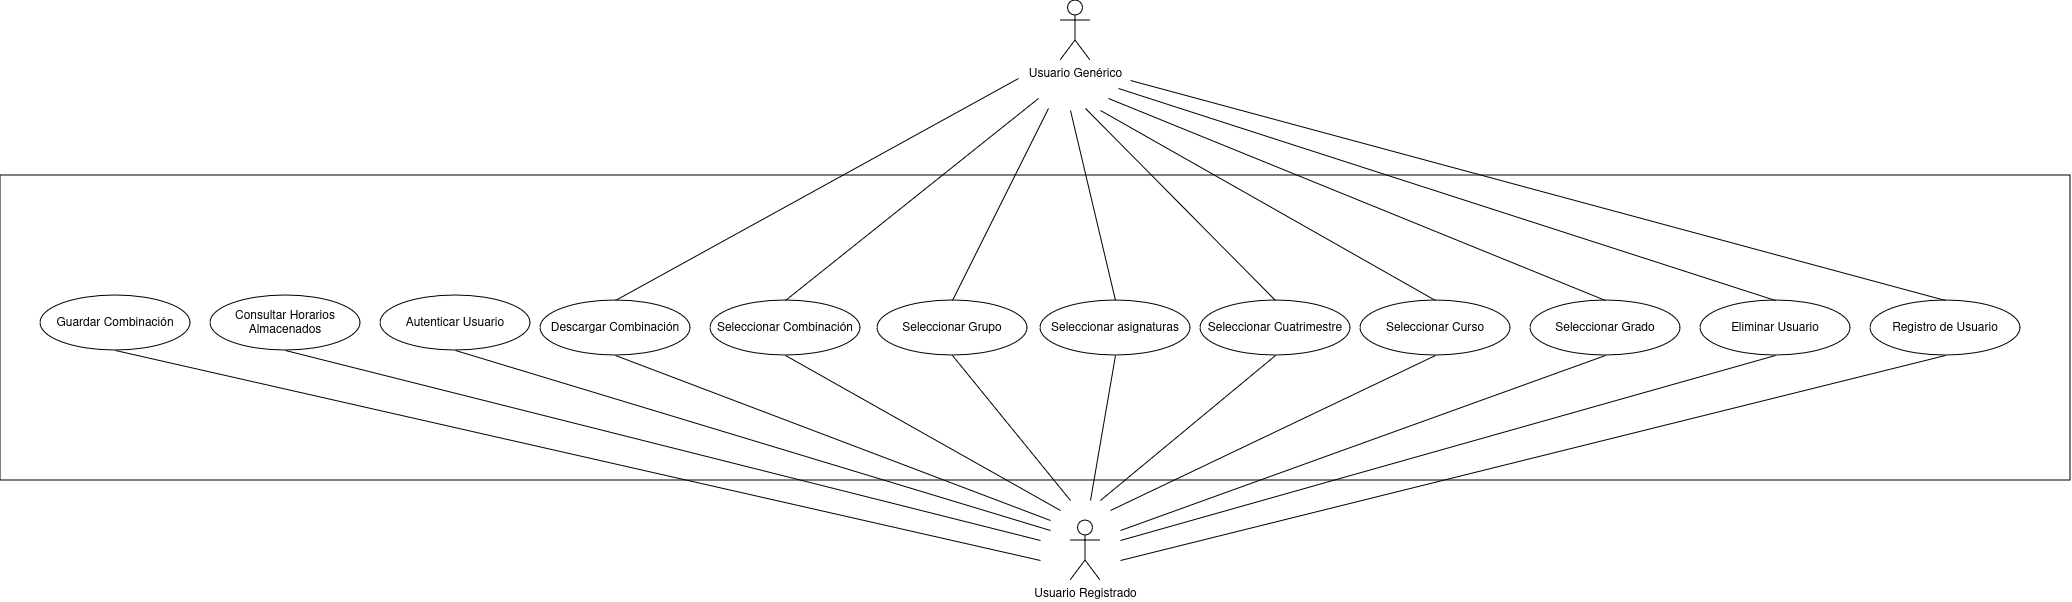
\includegraphics[width=1.9\textwidth]{./imagenes/CC_Actores_Comunes.png}
        \caption{Caso de Uso con Actores Comunes.}
    \end{figure}    
\end{landscape}

